\documentclass[aspectratio=169]{beamer}

% Tema utilizado. Também poderia ser:
%     Antibes       Darmstadt      Ilmenau         Marburg          Singapore
%     Bergen        Dresden        JuanLesPins     Montpellier      Szeged
%     Berkeley   [*]Frankfurt      Luebeck         PaloAlto         Warsaw 
%     Berlin        Goettingen     Madrid          Pittsburgh       boxes
%     Copenhagen    Hannover       Malmoe          Rochester        default

\mode<presentation>
{
  \usetheme{Frankfurt}
  \setbeamercovered{transparent}
}

\usepackage[portuguese]{babel}
\usepackage[utf8]{inputenc}
\usepackage{times}
\usepackage[T1]{fontenc}

%*****************
% CITATION OPTIONS
%*****************
\usepackage[citestyle=authoryear-comp, style=authoryear-comp, uniquename=false, maxcitenames=2, maxbibnames=9]{biblatex}
\renewcommand*{\nameyeardelim}{\addcomma\addspace}
\addbibresource{./referencias.bib}
\setbeamertemplate{caption}[numbered]
\beamertemplatenavigationsymbolsempty

%****************
% CAPTION OPTIONS
%****************
\usepackage{caption}
  \setbeamerfont{caption}{series=\normalfont,size=\fontsize{8}{10}} 
  \newcommand{\source}[1]{\caption*{Fonte: {#1}} }
  \setbeamertemplate{caption}[numbered]
  \setbeamercolor{caption name}{fg=structure!0!black}
  \let\oldparencite=\parencite
  \renewcommand{\parencite}[1]{\textcolor[rgb]{0,0,.6}{\oldparencite{#1}}}

%*********************
% JUSTIFY TEXT OPTIONS
%*********************  
\usepackage{ragged2e} 
  \addtobeamertemplate{block begin}{}{\justifying}
  \addtobeamertemplate{alertblock begin}{}{\justifying}

%**************
% BLOCK OPTIONS
%**************
\newenvironment<>{blockMargin10}[1]{%
 \begin{actionenv}#2%
 \def\insertblocktitle{\leftskip=10pt\rightskip=10pt\vspace{10pt} #1\vspace{10pt}}%
 \par%
 \usebeamertemplate{block begin}\leftskip=10pt\rightskip=10pt\vspace{10pt}}
 {\par\vspace{10pt}\usebeamertemplate{block end}
 \end{actionenv}}

 \newenvironment{variableblock}[4]{%
  \setbeamercolor{block title}{#2}
  \setbeamercolor{block body}{#3}
  \setbeamercolor{item projected}{#4}
  \begin{block}{#1}}{\end{block}}

%********************
% FOOTER TIKZ OPTIONS
%********************  
\usepackage{tikz}
  \tikzstyle{decision} = [
    diamond, 
    draw, 
    fill=blue!20, 
    text width=4.5em, 
    text badly centered, 
    node distance=3cm, 
    inner sep=0pt
  ]
\tikzstyle{block} = [
  rectangle, 
  draw, 
  thick,
  %fill=blue!20%, 
  text width=6em, 
  text centered, 
  rounded corners,
  minimum height=4em
]
\tikzstyle{line} = [
  draw, 
  -triangle 45
]
\tikzstyle{cloud} = [
  draw, 
  ellipse,fill=red!20, 
  node distance=3cm,
  minimum height=2em
]


\setbeamertemplate{footline}
{
    \leavevmode
    \hbox{
        \hspace{-2mm}
        \begin{beamercolorbox}[wd=.34\paperwidth,ht=2.5ex,dp=1.125ex,leftskip=.3cm plus1fill,rightskip=.3cm,center]{author in head/foot}
          \usebeamerfont{author in head/foot}\insertshortauthor
       \end{beamercolorbox}

      \begin{beamercolorbox}[wd=.33333\paperwidth,ht=2.5ex,dp=1.125ex,leftskip=.3cm,rightskip=.3cm plus1fil,center]{title in head/foot}
        \usebeamerfont{title in head/foot}\insertshortinstitute
      \end{beamercolorbox}

      \begin{beamercolorbox}[wd=.33333\paperwidth,ht=2.5ex,dp=1.125ex,leftskip=.3cm plus1fill,rightskip=.3cm]{author in head/foot}
        \usebeamerfont{title in head/foot}
        \insertframenumber{} / \inserttotalframenumber\hspace*{2ex}
      \end{beamercolorbox}
    }
    \vskip0pt
}
\makeatother 

\title[]{HLA e Microsserviços: Uma Aplicação para
Simulação Distribuída}

%\subtitle{Uma Exploração para Aplicabilidade em Cenários Operacionais}

\author[da Costa Neto et al]{
  Oswaldo Segundo da Costa Neto\inst{1}\\\and Carlos Magno Oliveira de Abreu\inst{2}\\\and Marcelo Alexandre Martins da Conceição\inst{1}\\\and André Benzi Baccarin\inst{1}\\\and Adilson Marques da Cunha\inst{1}
}

\institute[SIGE 2021]{
  \inst{1}%
  Instituto Tecnológico de Aeronáutica
  \and  
  \inst{2}%
  Centro de Análises de Sistemas Navais
}

\date[]{}

\subject{}

\pgfdeclareimage[height=0.6cm]{university-logo}{figs/sige.png}
\logo{\pgfuseimage{university-logo}}
\newcommand{\nologo}{\setbeamertemplate{logo}{}}

\AtBeginSection[]
{
  {
    \setbeamertemplate{footline}{} 
    \begin{frame}[noframenumbering]
      \frametitle{Roteiro}
      \tableofcontents[currentsection]
    \end{frame}
  }
}

%############################################################################
%##############################  INÍCIO  ####################################
%############################################################################

\begin{document}

%****************************************************************************
%                 CAPA
%****************************************************************************

\begingroup
  \setbeamertemplate{headline}[default]
  \begin{frame}[plain]
    \titlepage
    \vspace{-.8cm}
    \begin{figure}[ht!]
      \centering
      \includegraphics[width=.25\linewidth]{figs/sige-capa.png}
    \end{figure}
    \vspace{-.3cm}
  \end{frame}
\endgroup

%****************************************************************************
%                 OBJETIVO
%****************************************************************************

\begin{frame}{Objetivo}
  \begin{blockMargin10}{}
    Apresentar à audiência as possibilidades de desenvolvimento e execução de simulações distribuídas estruturadas no \textit{framework} HLA utilizando microsserviços. 
  \end{blockMargin10}
\end{frame}

%****************************************************************************
%                 ROTEIRO
%****************************************************************************

\begin{frame}[noframenumbering]
  \frametitle{Roteiro}
  \tableofcontents
\end{frame}

%****************************************************************************
%                 INTRODUÇÃO
%****************************************************************************
\section{Contextualização}
\begin{frame}{Contextualização}
  \begin{figure}[ht!]
    \centering
    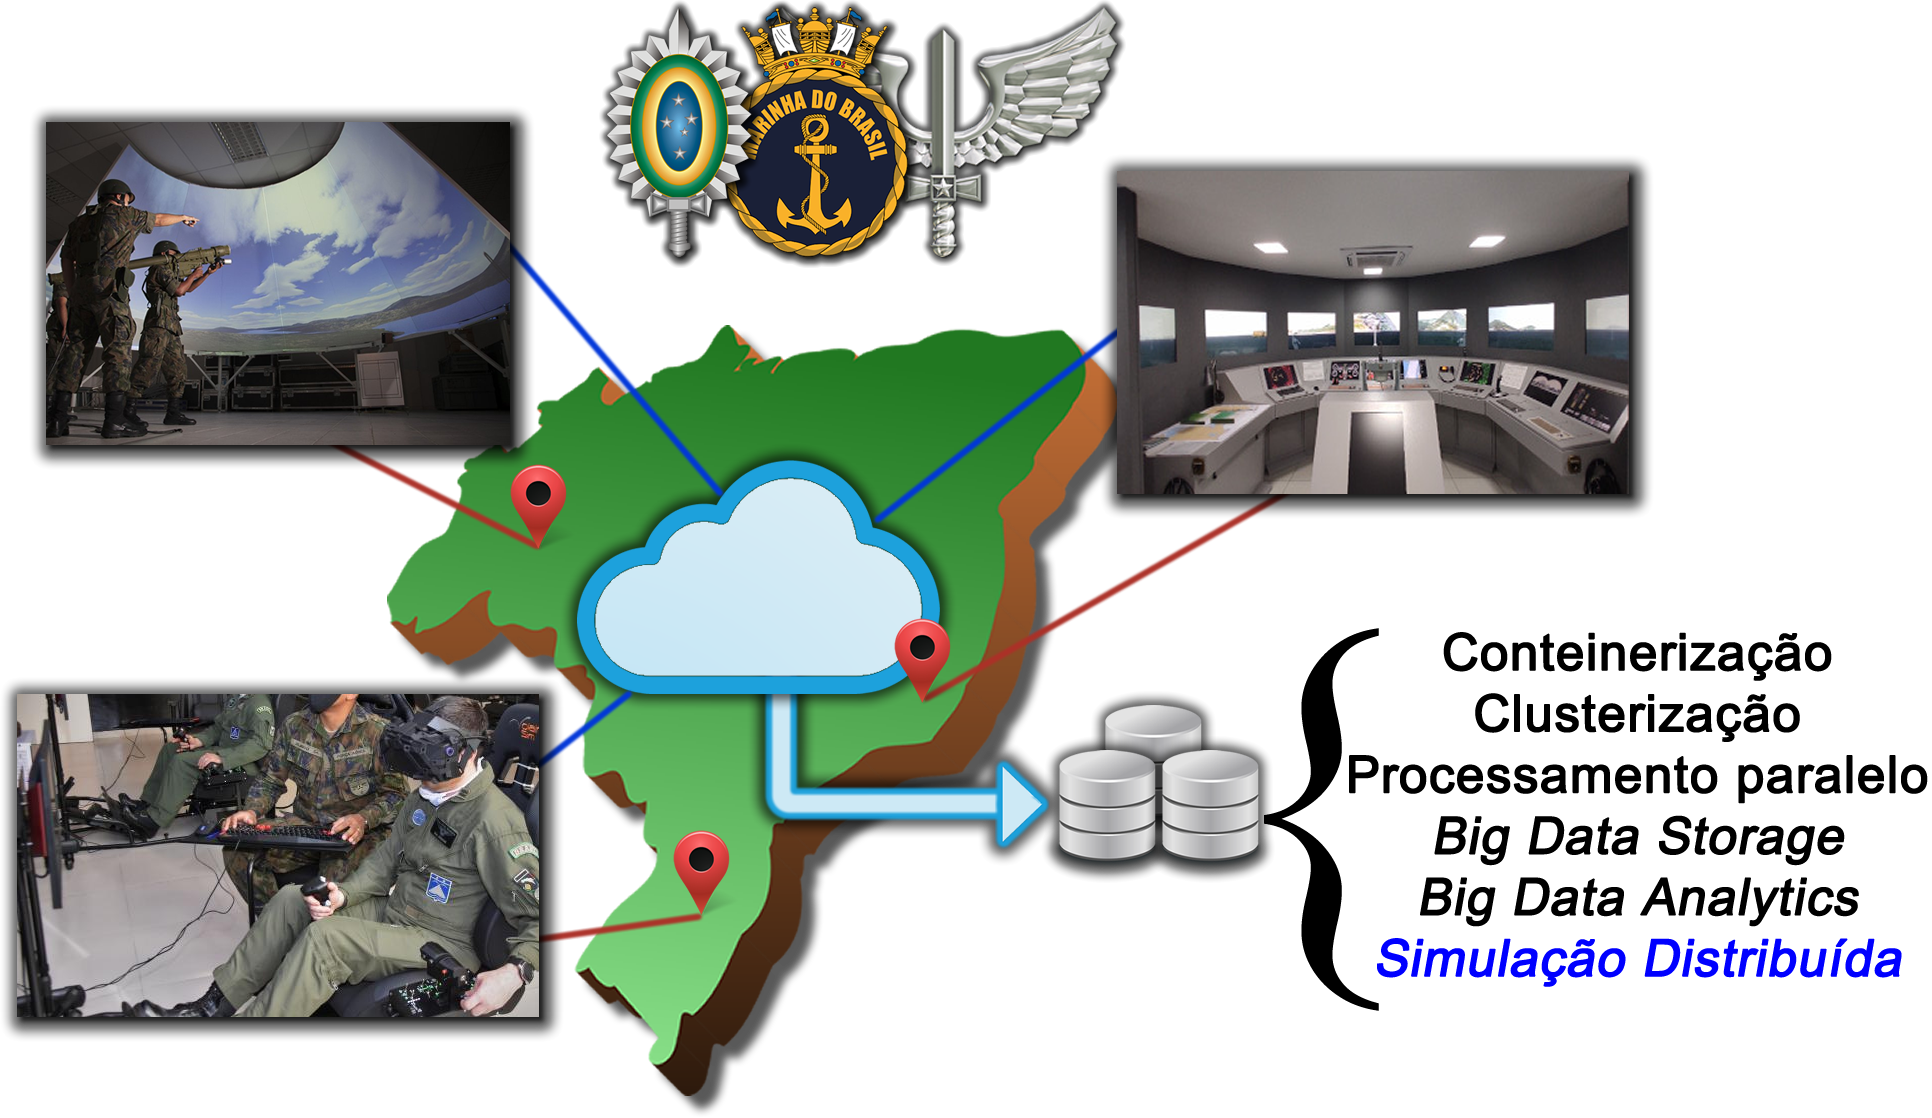
\includegraphics[width=.72\linewidth]{figs/cenario-atual.png}
    \caption{\centering Forças Armadas do Brasil utilizando o conceito de Simulação como um serviço}
  \end{figure}

  \note{
    \begin{itemize}
      \item \textbf{ESTA PESQUISA SE INSERE NESTE CONTEXTO\dots}
      \item Incentivo por parte do MD $\rightarrow$ DOU 2013
      \item Uma solução moderna $\rightarrow$ MSaaS
      \item Sem uma estrutura como essa ocorre:
      \begin{enumerate}
        \item Perda de capacidade de análise de Cenários Operacionais 
        \item Diminuição no potencial de treinamento 
      \end{enumerate}
    \end{itemize}
  }
\end{frame}

\begin{frame}{A Evolução das Arquiteturas de Simulação Distribuída}
  \begin{figure}[ht!]
    \centering
    \includegraphics[width=.8\linewidth]{figs/timeline.png}
    \caption{\centering Evolução das arquiteturas de Simulação Distribuída}
    \vspace{-0.5cm}
    \source{Adaptado de \parencite{Okan2017}}
  \end{figure}
  \note{
    \begin{itemize}
      \item \textbf{1970 - 1980}: Estudos iniciais promovidos pelo \textit{Department of Defense} (DoD) com objetivo de intercomunicar seus sistemas computacionais de simulação.
      \item \textbf{1984}: Projeto \textit{SIMulation NETworking} é iniciado, culminando com uma capacidade de conexão de 250 simuladores operando em 9 lugares distintos \parencite{Miller1995}.
      \item \textbf{1993}: Protocolos de comunicação do SIMNET se tornam padrão IEEE nomeado \textit{Distributed Interactive Simulation} (DIS).
      \item \textbf{1998}: Esforços contínuos liderados pelo DoD produziram um \textit{framework} para trazer uma facilitação na interoperabilidade entre os sistemas simulados. Era então criado o \textit{High Level Architecture} (HLA).
    \end{itemize}
  }
\end{frame}

\begin{frame}{Tendências de Padrões de Arquitetura}
  \begin{figure}[ht!]
    \centering
    \includegraphics[width=.7\linewidth]{figs/trending-simulation-architecture.png}
    \caption{\centering Tendências de uso de arquiteturas de Simulação Distribuída}
    \vspace{-0.5cm}
    \source{\parencite{Salio2012}}
  \end{figure}

  \note{

  }
\end{frame}

\begin{frame}{Topologias de Simulações Distribuídas}
  \centering
  \begin{columns}
    \begin{column}{.5\textwidth}
      \centering \textbf{DIS}
      \begin{figure}[ht!]
        \centering
        \includegraphics[width=.58\linewidth]{figs/Topology-parwise.png}
        \caption{\centering Topologia do tipo \textit{pair-wise integration}}
      \end{figure}
    \end{column}
    \begin{column}{.5\textwidth}
      \centering \textbf{HLA}
      \begin{figure}[ht!]
        \centering
        \includegraphics[width=1\linewidth]{figs/Topology-service-bus.png}
        \caption{\centering Topologia do tipo \textit{bus-service}}
      \end{figure}
    \end{column}
  \end{columns}

  \note{
    \begin{itemize}
      \item \textbf{DIS}: 
      \begin{enumerate}
        \item Tem uma topologia de comunicação direta entre os componentes. 
        \item É entendido como um protocolo de comunicação.
        \item PDU
        \item P2P
      \end{enumerate}
      \item \textbf{HLA}: 
      \begin{enumerate}
        \item Utiliza um barramento de comunicação.
        \item Proporciona melhor utilização do conceito de serviços. 
        \item \textit{Publish} / \textit{Subscribe}
        \item SOA
      \end{enumerate}
    \end{itemize}
  }
\end{frame}

%****************************************************************************
%                 CONCEITUALIZAÇÕES
%****************************************************************************
\section{Conceitualizações}

\begin{frame}{\textit{High Level Architecture} (HLA)}
  \vspace{-0.4cm}
  \only<1>{
    \begin{figure}[ht!]
      \includegraphics[width=.7\linewidth]{figs/rti.pdf}
      \vspace{-0.15cm}
      \caption{\centering Componentes de um cenário operacional a partir de uma Federação HLA}
    \end{figure}
  }
  \only<2>{
    \begin{figure}[ht!]
      \includegraphics[width=.7\linewidth]{figs/rti-fom.pdf}
      \vspace{-0.15cm}
      \caption{\centering Componentes de um cenário operacional a partir de uma Federação HLA}
    \end{figure}
  }

  \note<1>{

  }
  \note<2>{

  }
\end{frame}

\begin{frame}{\textit{High Level Architecture} (HLA)}

  \begin{columns}
    \begin{column}{.5\textwidth}
      \begin{figure}[ht!]
        \centering
        \includegraphics[width=1\linewidth]{figs/crc.pdf}
        \vspace{-.15cm}
        \caption{\centering Representação de uma RTI centralizada}
      \end{figure}
    \end{column}
    \begin{column}{.5\textwidth}
      \vspace{-.201cm}
      \begin{figure}[ht!]
        \centering
        \includegraphics[width=.66\linewidth]{figs/lrc.pdf}
        \vspace{.21cm}
        \caption{\centering Representação de uma RTI descentralizada}
      \end{figure}
    \end{column}
  \end{columns}
  
  \note{

  }
\end{frame}



\begin{frame}{Microserviços: Máquinas Virtuais X Docker}

  \begin{columns}
    \begin{column}{.5\textwidth}
      \begin{figure}[ht!]
        \centering
        \includegraphics[width=1\linewidth]{figs/estrutura-vm.pdf}
        \vspace{-.15cm}
        \caption{\centering Virtualização clássica com VMs}
      \end{figure}
    \end{column}
    \begin{column}{.5\textwidth}
      \begin{figure}[ht!]
        \centering
        \includegraphics[width=1\linewidth]{figs/estrutura-container.pdf}
        \vspace{-.15cm}
        \caption{\centering Virtualização \textit{lightweight} com \textit{containers}}
      \end{figure}
    \end{column}
  \end{columns}
  
  \note{

  }
\end{frame}

\begin{frame}{Microserviços}

  \begin{columns}
    \begin{column}{.5\textwidth}
      \begin{blockMargin10}{}
        \begin{itemize}
          \item Conteinerização de Federados HLA
          \item Orquestração e Coreografia
          \item Simulação como um serviço
          \item Interoperabilidade de Sistemas
        \end{itemize}
      \end{blockMargin10}
    \end{column}
    \begin{column}{.5\textwidth}
      \begin{figure}[ht!]
        \centering
        \includegraphics[width=1\linewidth]{figs/bridge.pdf}
        \vspace{-.15cm}
        \caption{\centering Rede Docker em Formato \textit{Bridge}}
      \end{figure}
    \end{column}
  \end{columns}
  
  \note{

  }
\end{frame}

%****************************************************************************
%                 ESTUDOS CORRELATOS
%****************************************************************************
\section{Estudos Correlatos}
\begin{frame}{Estudos Correlatos}
  \only<1>{
    \begin{figure}[ht!]
      \centering
      \includegraphics[width=.72\linewidth]{figs/rtiref.jpg}
      \caption{\centering Estrutura de Rede Aplicada em \parencite{VandenBerg2017}}
    \end{figure}
  }
  \only<2>{
    \begin{figure}[ht!]
      \centering
      \includegraphics[width=.72\linewidth]{figs/rtiref2.jpg}
      \caption{\centering Estrutura de Rede Aplicada em \parencite{VandenBerg2017}}
    \end{figure}
  }

  \note<1>{

  }
  \note<2>{
    
  }

  \note{
    \begin{itemize}
      \item \textbf{ESTA PESQUISA SE INSERE NESTE CONTEXTO\dots}
      \item Incentivo por parte do MD $\rightarrow$ DOU 2013
      \item Uma solução moderna $\rightarrow$ MSaaS
      \item Sem uma estrutura como essa ocorre:
      \begin{enumerate}
        \item Perda de capacidade de análise de Cenários Operacionais 
        \item Diminuição no potencial de treinamento 
      \end{enumerate}
    \end{itemize}
  }
\end{frame}


%****************************************************************************
%                 BIBLIOGRAFIA
%****************************************************************************

\appendix
\setbeamercolor{bibliography entry author}{fg=blue}
\setbeamercolor{bibliography entry title}{fg=black} 
\setbeamercolor{bibliography entry location}{fg=blue} 
\section{Apêndice}   
\begin{frame}[t, allowframebreaks]{Referências}
  \printbibliography
\end{frame} 

\end{document}



